
\subsection{Signatures}

\begin{figure}[!h]
	\centering
	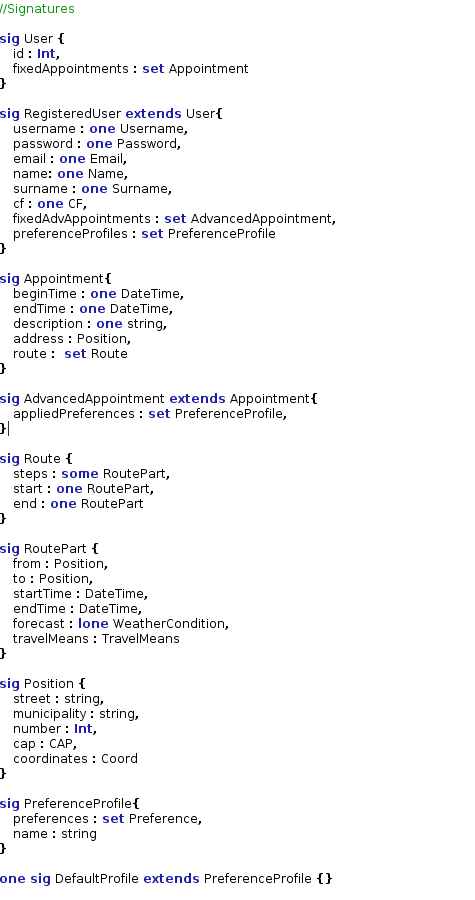
\includegraphics[height=\linewidth]{Images/Alloy/data.png}
	\caption{\label{fig:AlloySig1}Alloy signatures 1/2 }
\end{figure}

\begin{figure}[H]
	\centering
	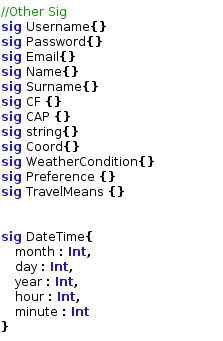
\includegraphics{Images/Alloy/data1.png}
	\caption{\label{fig:AlloySig2}Alloy signatures 2/2 }
\end{figure}

\subsection{Facts}

\begin{figure}
	\centering
	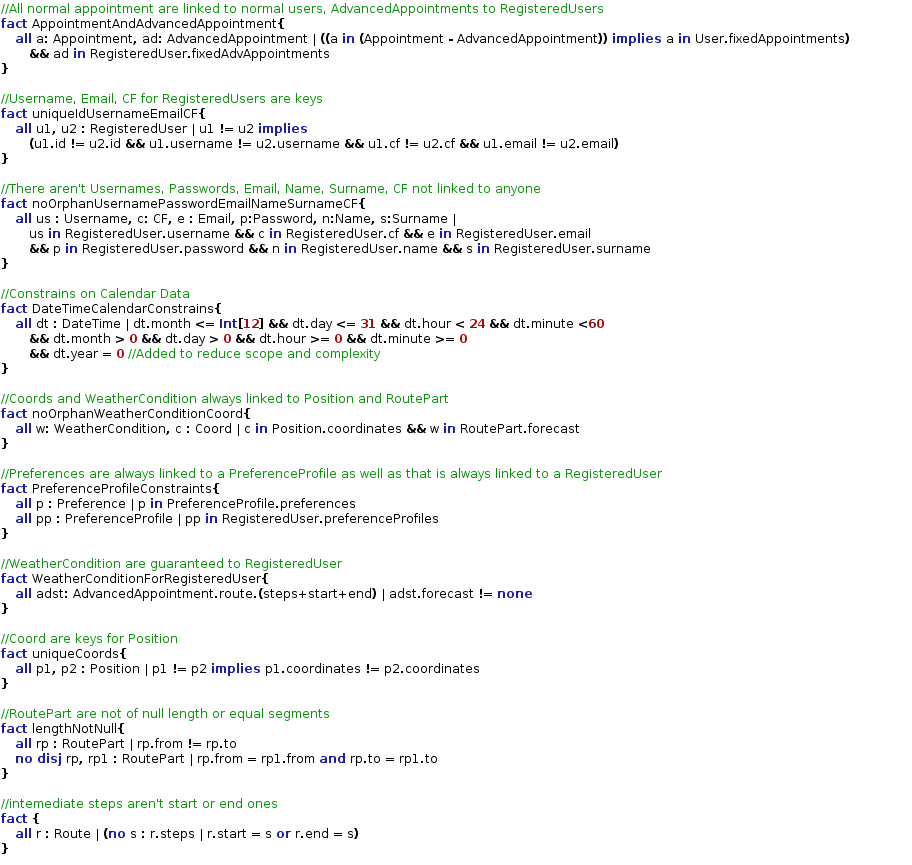
\includegraphics[width = \textwidth]{Images/Alloy/data2.png}
	\caption{\label{fig:AlloyFacts1}Alloy facts 1/2 }
\end{figure}

\begin{figure}[H]
	\centering
	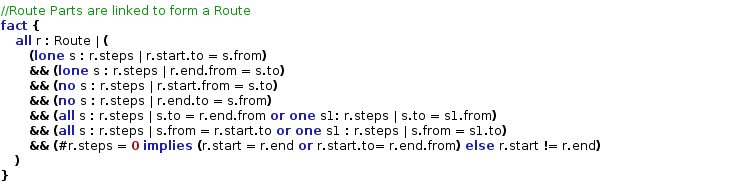
\includegraphics[width=\textwidth]{Images/Alloy/data3.png}
	\caption{\label{fig:AlloyFacts2}Alloy facts 2/2 }
\end{figure}

\subsection{Predicates}

\begin{figure}[H]
	\centering
	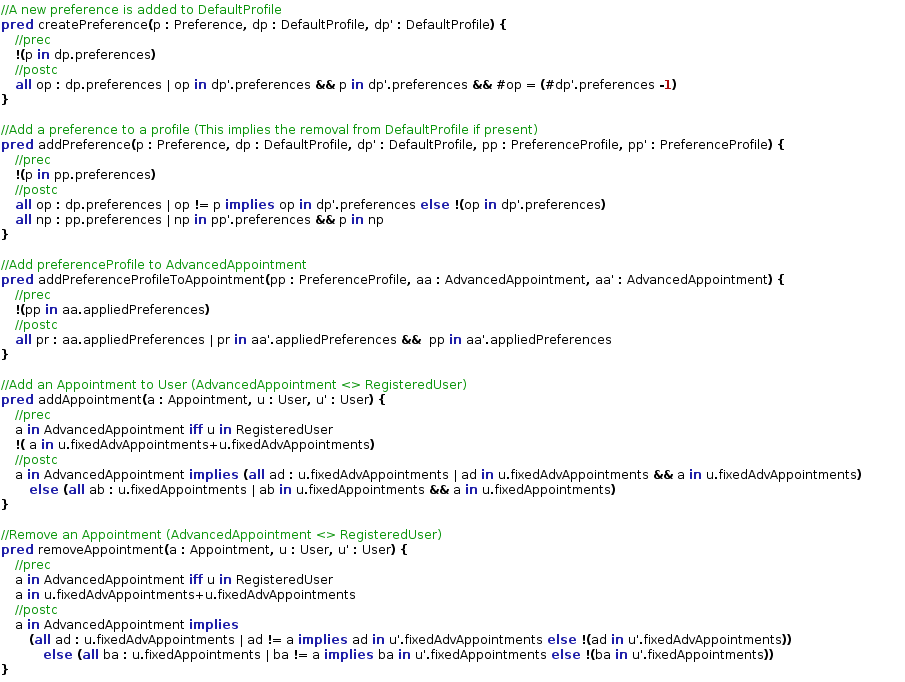
\includegraphics[width=\textwidth]{Images/Alloy/data4.png}
	\caption{\label{fig:AlloyPredicates}Alloy predicates }
\end{figure}

\subsection{Results}

\begin{figure}[H]
	\centering
	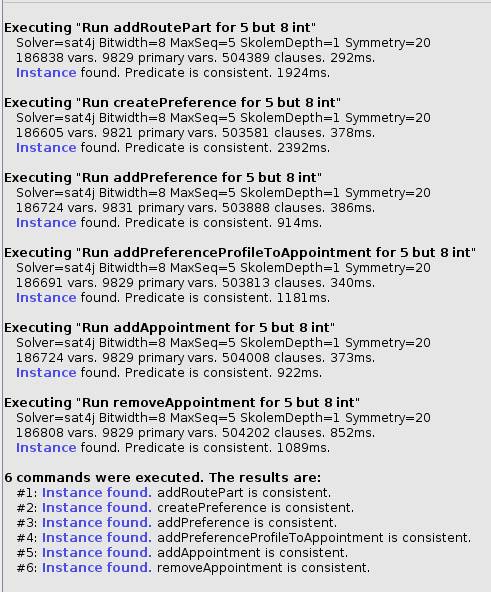
\includegraphics{Images/Alloy/data5.png}
	\caption{\label{fig:AlloyResults}Alloy consistency results }
\end{figure}

\subsection{World}

\begin{sidewaysfigure}
	\centering
	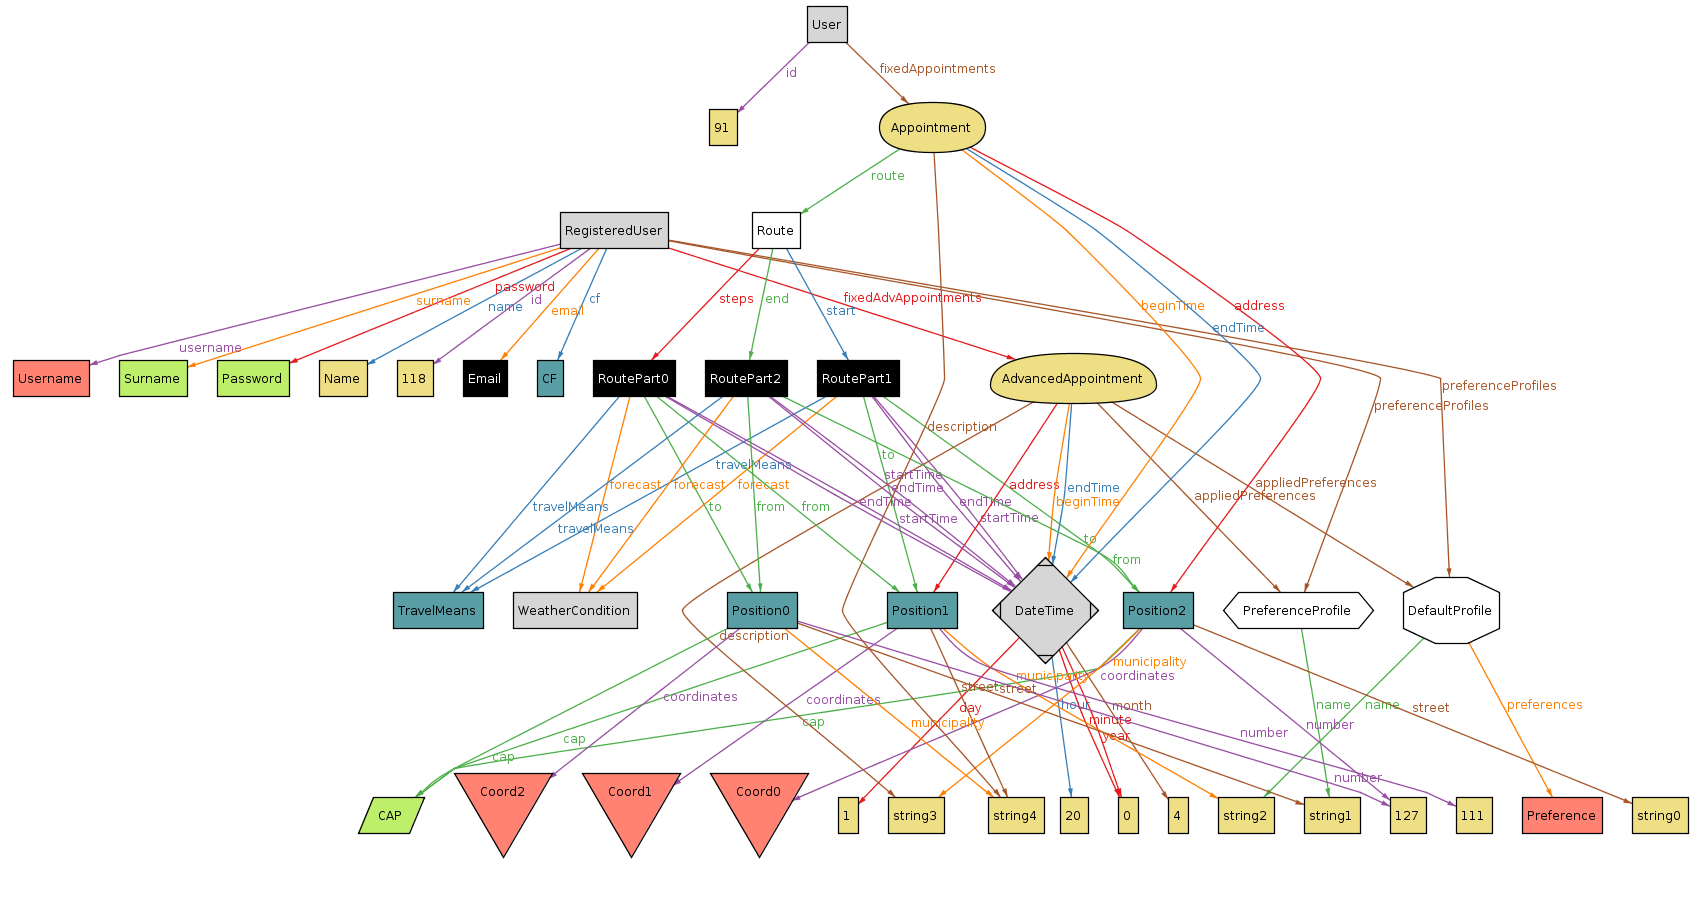
\includegraphics[width=\textwidth]{Images/Alloy/data6.png}
	\caption{\label{fig:AlloyWorld}Alloy generated world }
\end{sidewaysfigure}